\documentclass{beamer}
\usepackage{verbatim} % For using /begin{comment}; /end{comment}
%--------------------------------------------------------------%
\setlength{\parindent}{0em}
\setlength{\parskip}{0.5em}
\usepackage{graphicx}
\usepackage{mdwlist}
\definecolor{mine}{RGB}{155,155,155}
\definecolor{oj}{rgb}{1.0,0.65,0.0}
\definecolor{cblue}{rgb}{0.39, 0.58, 0.93}
\definecolor{turq}{rgb}{0.0, 0.81, 0.82}
%\usepackage{caption}
%\captionsetup[figure]{labelformat=empty}
\setlength{\unitlength}{1mm}

\setbeamercolor{normal text}{bg=black, fg=white}
\setbeamercolor{title}{fg=turq}
\setbeamercolor{frametitle}{fg=oj}
\setbeamercolor{block title}{fg=green}
\setbeamercolor{itemize item}{fg=mine} % all frames will have red bullets
\setbeamercolor{enumerate item}{fg=mine} % all frames will have red bullets

\usefonttheme{serif}
\setbeamerfont{frametitle}{series=\bfseries} % Frame titles should be bold

\title{Basic Principles of Solar Acoustic Holography}
\subtitle{ASTR 500}
\date{11 March 2016}
\author{Laurel Farris}

\begin{document}

%{\usebackgroundtemplate{\includegraphics[width=\paperwidth]
%{starwars.jpg}}
%\begin{frame}
%    \titlepage{}
%\end{frame}}
\begin{frame}
    \titlepage{}
    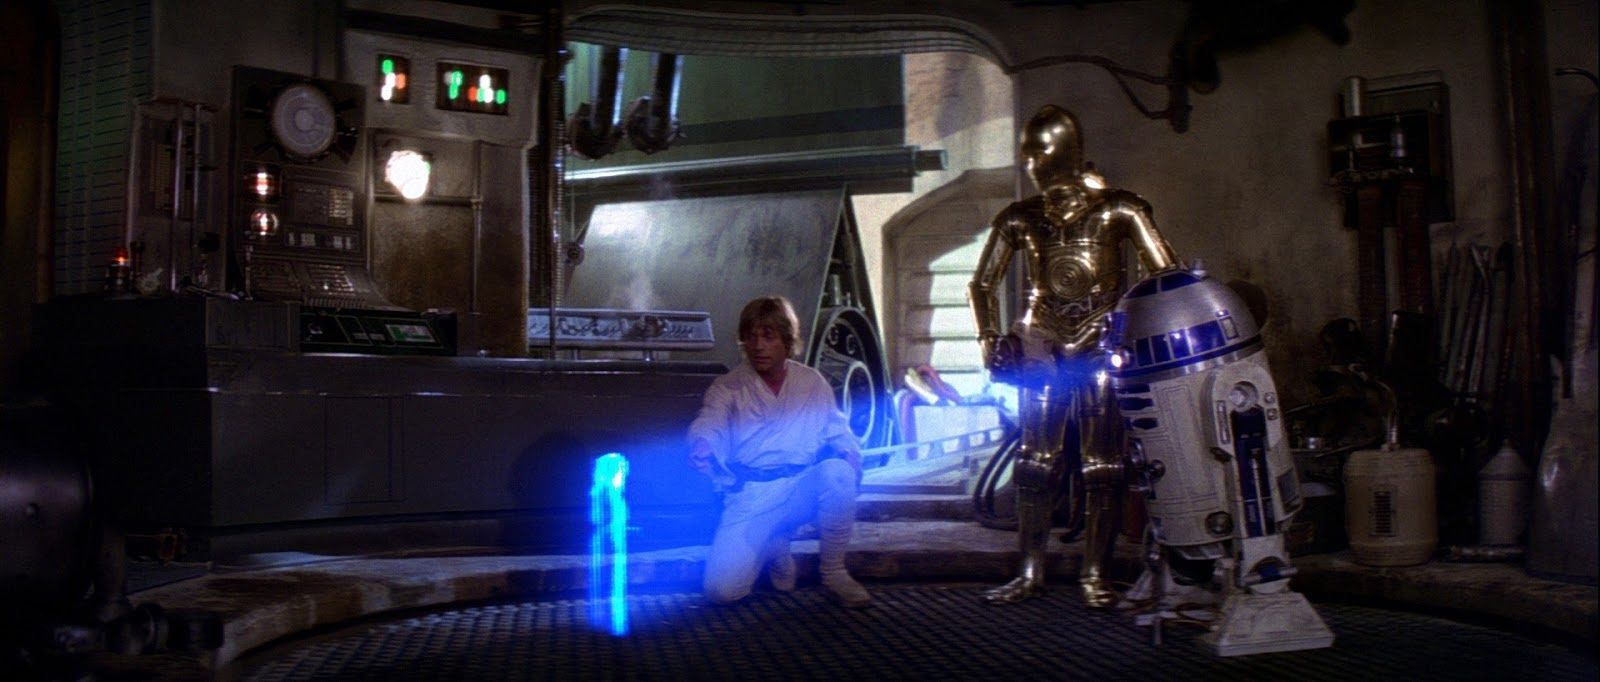
\includegraphics[width=\paperwidth]{starwars.jpg}
\end{frame}

\begin{frame}{Outline}
``Basic Principles of Solar Acoustic Holography''\\
C. Lindsey and D. C. Braun\\
2000
    \begin{enumerate}
        \item Introduction
        \item Basic Principles of Computational Seismic Holography
        \item The Computational Task
        \item Subjacent Vantage Holography
        \item An Example
        \item Acoustic Modelling Based on Holographic Images
        \item Phase-Sensitive Holography
        \item Green's Functions
        \item Summary
    \end{enumerate}
\end{frame}

\begin{frame}{Overview}
    Drawing on principles in optics and optical holography:
    \emph{Observe} the \emph{p}-mode spectrum, and extract
    information without using (possible incorrect) models.

    Comparing:
    \begin{itemize}
        \item simple acoustic-power
        \item phase-sensitive
    \end{itemize}
    Will eventually based solar models off of holographic signatures.

    Propose ``simple computational principles'' to produce images
    from observations.

    (Include some sort of eye diagram here?)

\end{frame}

\begin{frame}{1.1}
    ``Seismic holography'' was applied to helioseismic data from SOHO\@.
    ``New'' (1998-1999) solar acoustic phenomena:
    \begin{itemize}
        \item `acoustic moats' surrounding sunspots
        \item `acoustic condensations' 10-20 Mm beneath active regions
        \item `acoustic glories' surrounding complex active regions
        \item first helioseismic images of a flare
    \end{itemize}
    $\rightarrow$ solar cycle dependence of global \emph{p}-modes!
    (which is $\ldots$ ?)

    Magnetic regions reflect \emph{p} modes above the acoustic cutoff
    frequency, where the surface of the \emph{quiet} sun ($\sim$ 10 G)
    acts as a nearly perfect absorber of incident acoustic radiation
    coming from the sun's interior.
\end{frame}

\begin{frame}{1.2 \- The Basic Principle}
    The \emph{phase-coherent} (what does this mean?) computational
    reconstruction of the \emph{acoustic field} in the solar interior,
    so that \emph{stigmatic images} (what are these?) of the sources
    of these disturbances can be produced.

    Historical info here that might go in a pre-paper slide.
\end{frame}

\begin{frame}{1.3}
    \begin{itemize}
        \item Concept proposed in 1975 by Roddier
        \item Developed over the 1990s by Lindsey and Braun
            (current authors)
        \item Key to locating and examining fine structure as deep as
            possible.
    \end{itemize}
\end{frame}

\begin{frame}{1.4}
Seismology and tomography are not the same thing! Tomography is great
for X-ray applications in the medical field, not so good for
astronomical seismology; poor statistics and diffraction limited resolution.
Holography is definitely not just another method of \emph{modeling}
stellar interiors, the images provide more of a basis for modeling
techniques.
\end{frame}

\begin{frame}{1.5}
Helioseismic holography defined in terms of seismic imaging by
phase-coherent reconstruction of the acoustic field into the solar
interior. The terms `seismic imaging' and `helioseismic imaging' are
applied in a broader context to include \emph{partially} coherent
acoustic signatures suggested to appear at the antipodes of far-side
acoustic absorbers. `Holographic' seismology applies to near side, far
side, and everything in between.
\end{frame}

\begin{frame}{Part 2: Basic Principles of Computational Seismic
Holography}
\end{frame}

\begin{frame}{2.1; Figure 1}
    \begin{figure}
        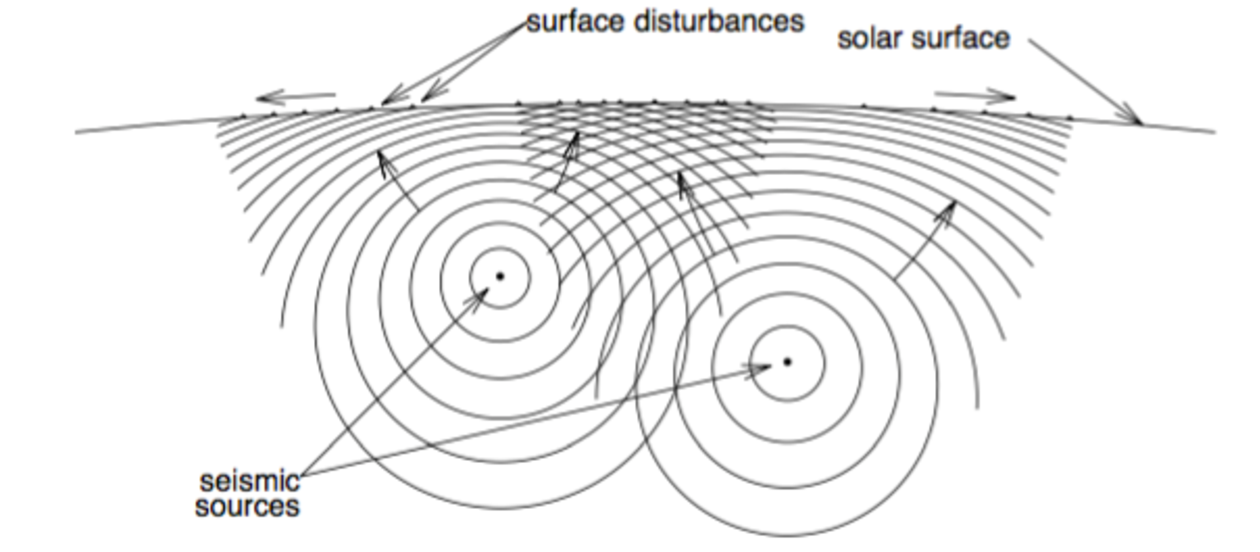
\includegraphics[width=0.8\textwidth]{fig_1.pdf}
    \end{figure}
    \begin{itemize}
        \item Well-defined acoustic sources
        \item All we see is the pattern of ripples at the surface,
            propagating from points directly \emph{above} the sources.
        \item The waves are absorbed upon reaching the surface
            (accurate for $\nu >\ \sim 5.5$ mHz (what's the significance of
            this??)
    \end{itemize}
\end{frame}

\begin{frame}{2.2; Figure 2}
    \begin{figure}
        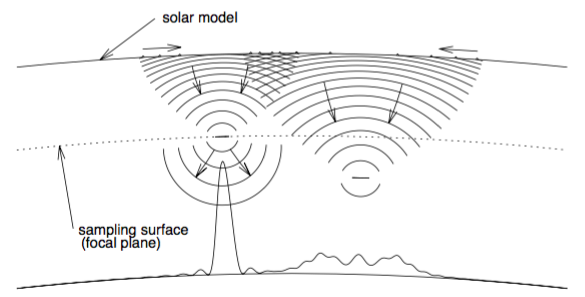
\includegraphics[width=0.8\textwidth]{fig_2.png}
    \end{figure}
    \begin{itemize}
        \item Apply time-series of observations to model with no
            sources, sinks, or scattering (of what?)
        \item The observances are ``seen'' at the ``pupil''.
        \item Place the ``focal plane'' at the location of the
            sources, and get a diffraction-limited signature
            (left side of figure).
        \item If focal plane is above or below the source, we get an
            unfocused, diffuse profile (right side of figure).
    \end{itemize}
\end{frame}

\begin{frame}{2.3; Figure 3}
    \begin{itemize}
        \item Simulation: random acoustic noise in model that
            contains alphanumeric absorbers at six different locations,
            from just below the surface to a depth of 56 Mm
            ($\sim \frac{1}{10}$ R$_{\odot}$).
        \item `acoustic stalactite' of the aborber \- the de-focused
            plume.
        \item a diffuse `stalagmite' appears closer to the absorber
        \item sharp, diffraction-limited silhouette at 56 Mm.
        \item depth diagnostics accomplished by focusing and
        de-focusing, rather than the appearance or disappearance that
        would be used in realistic phyiscal models.
    \end{itemize}
    \begin{figure}
        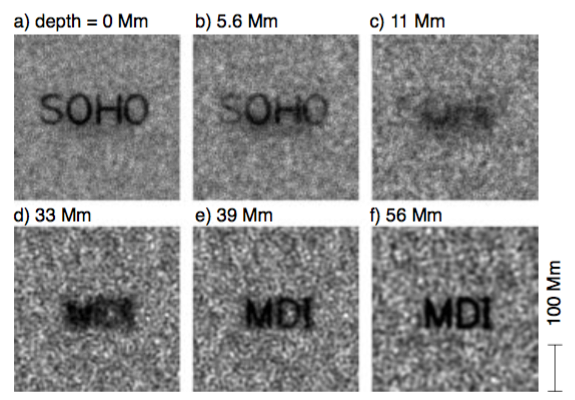
\includegraphics[width=0.8\textwidth]{fig_3.png}
    \end{figure}
\end{frame}

\begin{frame}{2.4}
Seismic holography is most certainly not a representation of solar
acoustics in terms of ray optics. These are mechanical waves, not
electromagnetic ones, though they have similiar behavior, such as
interference and diffraction. Thus, it suffers from the same
limitations as other helioseismological observations, and the same
kind of optimization techniques used to extract information from
coherent electromagnetic radiation can also be used here.
\end{frame}

%-------------------------------------------------------------------%
\begin{frame}{Part 3: The Computational Task}
\end{frame}

\begin{frame}{3.1}
    Two perspectives:
    \begin{enumerate}
        \item the ``spectral'': the disturbance in terms of the normal
            modes of the medium
        \item the ``time distance'': closer to that of time-distance
            helioseismology
    \end{enumerate}
    Terms used:
    \begin{itemize}
        \item space-time
        \item wavenumber-frequency
    \end{itemize}
\end{frame}

\begin{frame}{3.2}
    Given
    \begin{itemize}
        \item acoustic amplitude
        \item its derivative
    \end{itemize}
    can extrapolate the acoustic field anywhere in the interior!
    Although it's incomplete; we're getting a significant fraction, but not
    the entire interior. Future terminology:
    \begin{itemize}
        \item $H$ - incomplete regression of the acoustic field
        \item $\psi$ - Actual acoustic field
    \end{itemize}
\end{frame}

\begin{frame}{3.3: The space-time perspective}

    $\psi(\mathbf{r}',t')$ - acoustic field, secured at time
    $t'$ and horizontal location $\mathbf{r}'$
    regression is expressed by a formalism called the ``acoustic egression'',
    $H_{+}(\mathbf{r},z,t)$, an imcomplete, but coherent assessment of the local
    acoustic disturbance that has emanated from the ``focal point'',
    $(\mathbf{r},z)$, of the computation at time $t$ based on its succeeding
    emergence at the overlying surface over the range of locations and time
    expressed by $(\mathbf{r}',0,t')$. This can be expressed by an integral
    of the form:
    $$ H_{+}(\mathbf{r},z,t) = \int
    \textrm{d}t' \int\limits_{a<|\mathbf{r}-\mathbf{r}'|<b}
    \textrm{d}^{2}r'G_{+}
    (|\mathbf{r}-\mathbf{r}'|,z,t-t')\psi(\mathbf{r}',t')  $$
    $G_{+}$ - Green's function that expresses how a single transient point
    disturbance propagates forward or backward in time between
    $(\mathbf{r}',0,t')$ and $(\mathbf{r},z,t)$.
\end{frame}

\begin{frame}{3.4}
    $H_{-}$ - acoustic ingression, time reverese of $H_{+}$.
    Describes waves coherently converging into a point, rather than from it.
    Replace $G_{+}$ by its time reverse:
    $$ G_{-}(|\mathbf{r}-\mathbf{r'}|,z,t-t') =
    G_{+}(|\mathbf{r}-\mathbf{r'}|,z,t'-t) $$
    \begin{picture}(60,40)
        % first circle
        \put(20,20){\circle{20}}
        \put(20,20){\circle{10}}
        \put(20,20){\vector(3,0){7}}
        \put(20,20){\vector(0,5){10}}
        % second circle
        \put(60,20){\circle{20}}
    \end{picture}
\end{frame}

\begin{frame}{3.5}
    After computing $H_{+}$, square and integrate it to produce an egression
    power map over the time period in desired range.
    \emph{p}-mode absorption in sunspots has already been confirmed this way!
\end{frame}

\begin{frame}{3.6: The wavenumber-frequency perspective}
    \begin{itemize}
        \item $\hat{\psi}(\mathbf{k},\nu)$ - Fourier transform of $\psi(\mathbf{r},t)$
        \item $\hat{G}_{+}(|\mathbf{k}|,z,\nu)$ - Fourier transform of
            $G_{+}(|\mathbf{r}|,z,t)$
    \end{itemize}
    From the convolution theorem:
    $$ \hat{H}_{+}(\mathbf{k},z,\nu) = \hat{G}_{+}(|\mathbf{k}|,z,\nu),
     \hat{\psi}(\mathbf{k},\nu) $$
   Multiplication is computationally \emph{faster} than convolution, so this
   perspective is used henceforth.
\end{frame}

\begin{frame}{3.7}
Start getting aberrations; some are easily corrected (e.g.\ spherical
aberration, distortion, and curvature of field). Some however, are not
(coma, primary astigmatism, and higher order aberrations) for large
pupils that are needed to form deep focal planes (deep sources), or
for imaging the far side of the sun. In this case, the
aforementationed wavenumber perspective cannot be used.
\end{frame}

\begin{frame}{3.8}
$$ \check{H}_{+}(\mathbf{r},z,\nu) =
\int\limits_{a<|\mathbf{r}-\mathbf{r}'|<b}\textrm{d}^{2}r'\check{G}_{+}
    (|\mathbf{r}-\mathbf{r}'|,z,\nu)\check{\psi}(\mathbf{r}',\nu) $$
\end{frame}

%-------------------------------------------------------------------%
\begin{frame}{Part 4: Subjacent Vantage Holography}
\end{frame}

\begin{frame}{Figure 4}
    \begin{figure}
        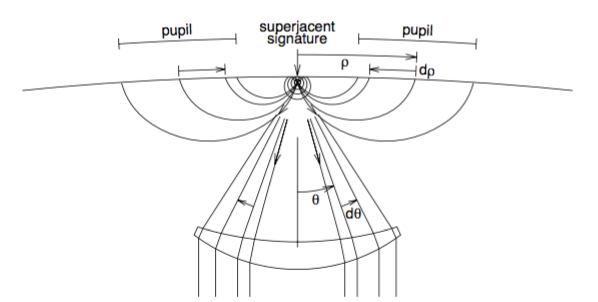
\includegraphics[width=0.8\textwidth]{fig_4.png}
    \end{figure}
\end{frame}

\begin{frame}{4.1}
    Previously: ``\emph{Super}jacent vantage Holography''.
    \emph{Sub}jacent vantage holography is when the inner radius, $a$,
    of the pupil annulus is much greater than the depth of the focal plane
    (where the source is). This usually applies to quiet sun areas, whereas
    the superjacent vantage applies to active regions.
\end{frame}

\begin{frame}{4.2}
    In contrast to normal optics, the diffraction limit is set by how
    compact the inner radius is.
\end{frame}

\begin{frame}{4.3}
    (Explains which panels in figure 3 are sub or superjacent)
\end{frame}

%-------------------------------------------------------------------%
\begin{frame}{Part 5: An Example}
\end{frame}

\begin{frame}{5.1}
\end{frame}

\begin{frame}{Figure 5}
    \begin{figure}
        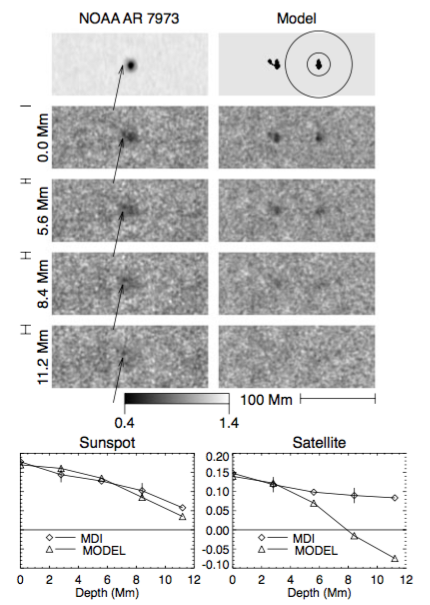
\includegraphics[width=0.8\textwidth]{fig_5.png}
    \end{figure}
\end{frame}

\begin{frame}{5.2}
\end{frame}

\begin{frame}{5.3}
\end{frame}

\begin{frame}{5.4}
\end{frame}

\begin{frame}{5.5}
    Fundamental limitation: As sound speed increases with depth, wavelength
    \emph{increases}, which results in a coarser diffraction limit at
    any frequency.
\end{frame}

\begin{frame}{Part 6: Acoustic Modeling Based on Holographic Images}
\end{frame}

\begin{frame}{6.1}
    Applying phase-sensitive holography to models:
    Flexible procedures, such as inversions, would characterize the
    acoustic environment in pysical terms such as:
    \begin{itemize}
        \item acoustic emissivity
        \item acoustic opacity
        \item refractivity
        \item flow velocity
    \end{itemize}
\end{frame}

\begin{frame}{6.2}
    $$ \langle|H_{+}(\mathbf{r},z)|^{2}\rangle =
    \int\textrm{d}^{2}\mathbf{r}'\int\textrm{d}z'g^{-1}
    (|\mathbf{r}-\mathbf{r}'|,z,z')S(\mathbf{r}',z') $$
\end{frame}

\begin{frame}{Part 7: Phase-Sensitive Holography}
\end{frame}

\begin{frame}{7.1}
\end{frame}

\begin{frame}{7.2}
    The need for phase-sensitive holography is two-fold:
    \begin{enumerate}
        \item straight-forward quantitative probe of refractive anomalies
            that we expect from thermal perturbations
        \item ?
    \end{enumerate}
\end{frame}

\begin{frame}{7.3}
    Visualize phase-sensitive holography in terms of a \emph{gedanken experiment}.
    \begin{itemize}
        \item No phase-shift
        \item Phase-shift:\\
            \begin{itemize}
                \item $\Delta{n} = \Delta{c}/c \rightarrow$
                    refractive perturbation
                \item $\Delta{t} \sim a\Delta{n}/c \rightarrow$
                    time delay
                \item $\Delta{\phi} \sim 2\pi\nu a\Delta{n}/c \rightarrow$
                    phase shift
            \end{itemize}
    \end{itemize}
\end{frame}

\begin{frame}{Figure 6}
    \begin{figure}
        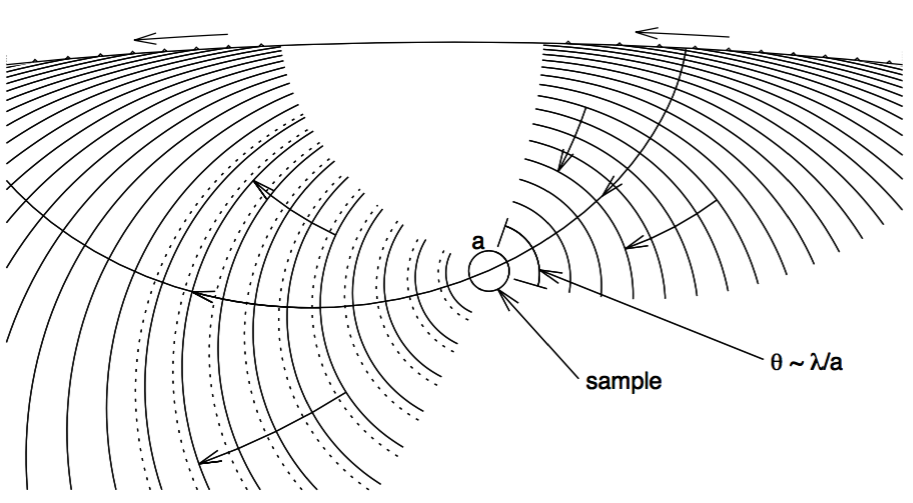
\includegraphics[width=0.8\textwidth]{fig_6.png}
    \end{figure}
\end{frame}

\begin{frame}{Part 8: Green's Functions}
\end{frame}

\begin{frame}{8.1}
    Green's function:
    $$ G_{\pm}(|\mathbf{r}-\mathbf{r}'|,z,t-t') $$
    Characterizes the acoustics of the solar \emph{model}
    to which helioseismic observations,
    $\psi(\mathbf{r}',t')$,
    are applied to accomplish acoustic regressions.

    Computational is a broad, flexible diagnostic,
    not intended for any one particular model.

    Outlining intuitive concepts used to fashion Green's Functions
    appropriate for practical diagnostic applications.
\end{frame}

\begin{frame}{8.2}
    Acoustic formalism:
    \begin{itemize}
        \item Field, $\psi$ is normalized wrt energy flux
        \item Solar inteior acoustics (in the absense of sources
            and sinks) is \emph{time-reversal invariant}
    \end{itemize}
    Given these two conditions, the same Green's functions characterize
    the propagation both forward and backward in time between surface
    $(\mathbf{r}',0,t')$ and source $(\mathbf{r},z,t)$
\end{frame}

\begin{frame}{8.3: Dispersionless acoustics}
    Pulse propagates in the form of a \emph{wavefront}.
    Surface location, $\mathbf{r}'$ responds with ripple characterized
    by the same infinitely sharp temporal profile as the source,
    but properly attenuated. The Green's function is invarient with
    respect to both time and horizontal translation.
    $$ G_{+}(|\mathbf{r}-\mathbf{r}'|,z,t-t') =
    \delta\left(t-t'-T\left(|\mathbf{r}-\mathbf{r}'|,z\right)\right)
       f\left(|\mathbf{r}-\mathbf{r}'|,z\right)$$
\end{frame}

\begin{frame}{8.4}
\end{frame}

\begin{frame}{8.5}
    $T$ (travel time) and $f$ (amplitude of pulse) both depend
    strongly on the sound speed variation with depth.
    Derive $\Gamma$ (optimal optical path) that satisfies
    Fermat's principle.

    Obtain $T$!
\end{frame}

\begin{frame}{8.6}
    Obtain $f$; acoustic flux must be in proportion to solid angle
    subtended by the optical paths leading to the boundary of the
    surface element.

    Acoustic energy flux density: $cf^{2}$
\end{frame}

\begin{frame}{Figure 7}
    \begin{figure}
        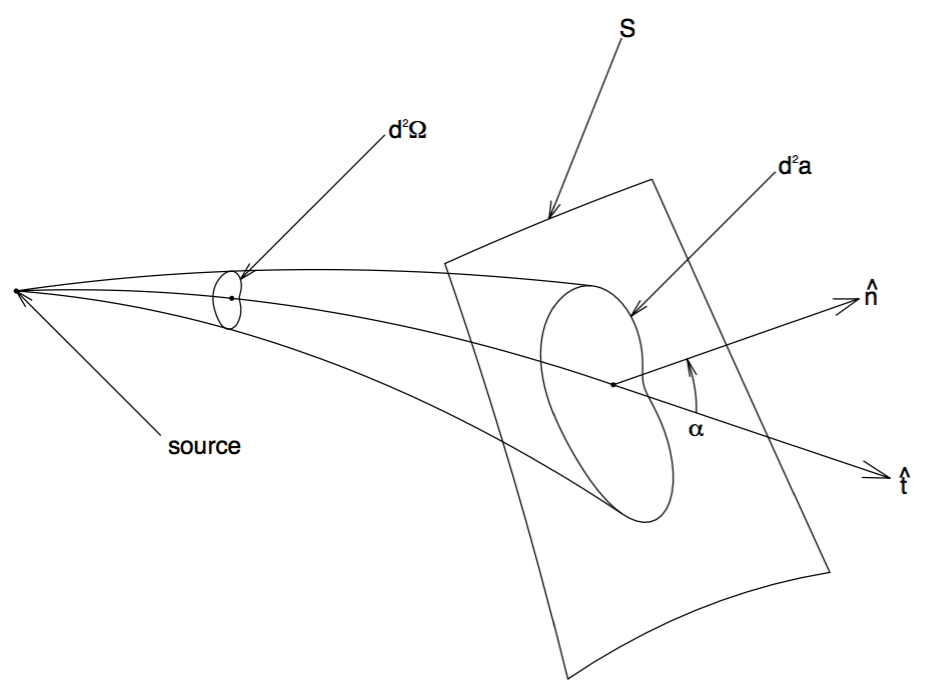
\includegraphics[width=0.8\textwidth]{fig_7.png}
    \end{figure}
\end{frame}

\begin{frame}{8.7}
    \begin{itemize}
        \item $\nu>5.5$ mHz absorbed by photosphere upon first
            encounter after leaving source.
        \item $\nu<4.5$ mHz reflected from the specular
            (``mirror-like''). In this case the Green's function
            is characterized by a sum of $n$ components, where
            each $n$ is a ``skip'', or reflection from the photosphere
            (include diagram)
    \end{itemize}
\end{frame}

\begin{frame}{8.8}
    Multiple-skip holography: Two branches
    \begin{enumerate}
        \item $\rho$ decreases as $\theta$ increases
        \item $\rho$ increases after reaching a minimum as $\theta$
            continues to increase toward 180$^{\circ}$.
    \end{enumerate}
\end{frame}

\begin{frame}{Figure 8}
    \begin{figure}
        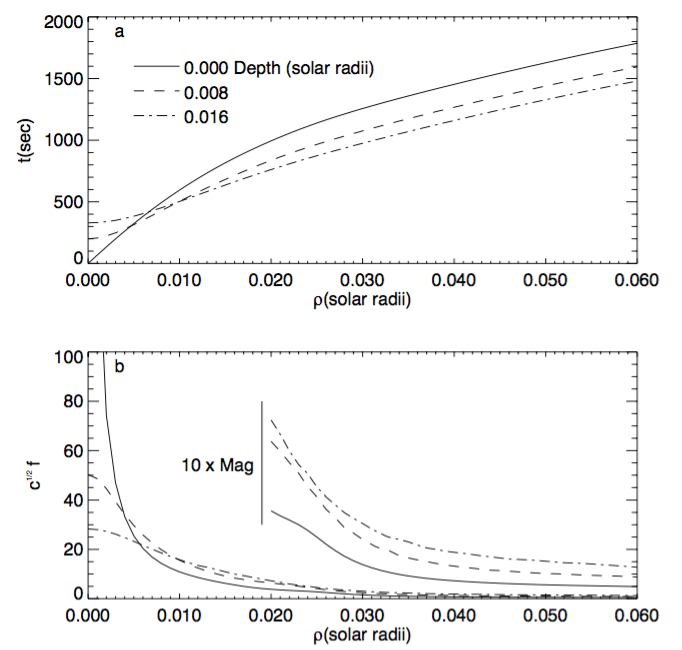
\includegraphics[width=0.8\textwidth]{fig_8.png}
       % \caption{captiontext}
       % \label{figurelabel}
    \end{figure}
\end{frame}

\begin{frame}{Figure 9}
    \begin{figure}
        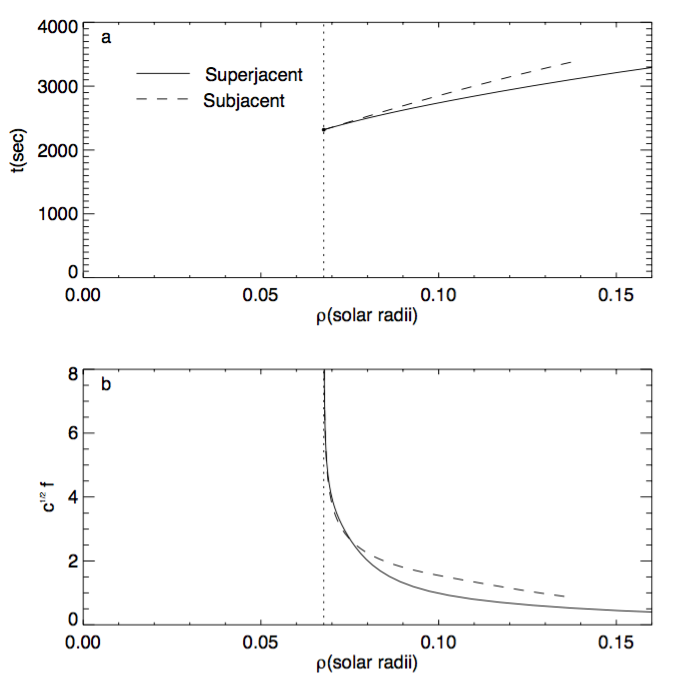
\includegraphics[width=0.8\textwidth]{fig_9.png}
       % \caption{captiontext}
       % \label{figurelabel}
    \end{figure}
\end{frame}

\begin{frame}{8.10: Dispersion}
    In reality, acoustic waves are \emph{significantly} dispersed
    near the photosphere.
\end{frame}

\begin{frame}{8.9}
\end{frame}

\begin{frame}{8.11}
\end{frame}

\begin{frame}{8.12}
\end{frame}

\begin{frame}{8.13}
\end{frame}

\begin{frame}{8.14}
\end{frame}



\begin{frame}{Figure 10}
    \begin{figure}
        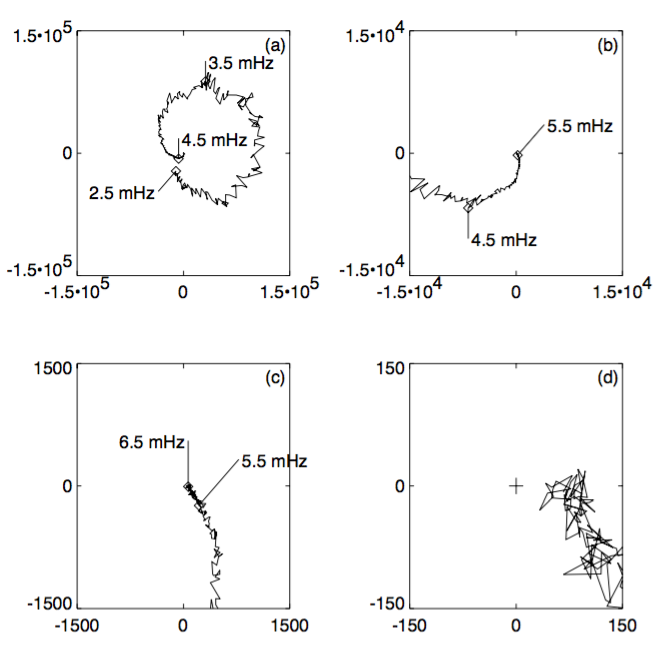
\includegraphics[width=0.8\textwidth]{fig_10.png}
       % \caption{captiontext}
       % \label{figurelabel}
    \end{figure}
\end{frame}

\begin{frame}{Figure 11}
    \begin{figure}
        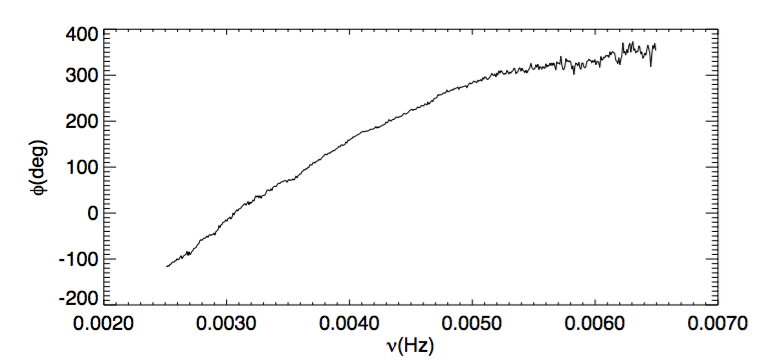
\includegraphics[width=0.8\textwidth]{fig_11.png}
       % \caption{captiontext}
       % \label{figurelabel}
    \end{figure}
\end{frame}

\begin{frame}{Part 9: Summary}
\end{frame}

%--------------------------------------------------------------%

\end{document}
